\section{Prise en main d'un modèle de processeur}
\label{sec:processeur}

Le processeur fourni sur Madoc (\texttt{riscvproc-2.v}) est un modèle comportemental Verilog qui
implémente une partie du jeu d'instructions RV32I~\cite{riscvspec} : \texttt{add},
\texttt{sub}, \texttt{sll}, \texttt{srl}, \texttt{addi}, \texttt{andi}, \texttt{ori},
\texttt{lw}, \texttt{sw} et \texttt{ebreak}. Il contient une mémoire interne \texttt{memory} de
4096 mots de 32 bits, qui sert à la fois au programme et aux données, ainsi que les 32 registres
\texttt{x0} à \texttt{x31}. Une instruction est exécutée toutes les \texttt{Step} = 10~ns ; le
module \texttt{system} n'a aucun port, c'est un modèle purement simulable.

Le fichier utilise des constructions SystemVerilog (\texttt{localparam int unsigned}) : nous
l'avons renommé avec l'extension \texttt{.sv} et compilé avec \texttt{vlog -sv}. L'instruction
\texttt{ebreak} termine la simulation par \texttt{\$finish} ; nous lançons donc \texttt{vsim}
avec l'option \texttt{-onfinish stop}, qui arrête la simulation sans fermer le design et permet
d'examiner ensuite les registres et la mémoire.

% ---------------------------------------------------------------------------
\subsection{Valider le processeur RISC-V}
\label{sec:validation}

Pour faire exécuter un programme, la mémoire du processeur est initialisée au début de la
simulation à partir d'un fichier texte, avec la tâche système \texttt{\$readmemh} placée dans le
bloc \texttt{initial} du processeur (code~\ref{lst:readmemh}). Le fichier contient un mot de
32 bits en hexadécimal par ligne ; \texttt{@0} donne l'adresse du premier mot et \texttt{//}
introduit un commentaire. Le chemin est relatif au répertoire courant de ModelSim : si le
fichier n'est pas trouvé, ModelSim l'indique par un avertissement, la mémoire reste à
\texttt{X} et le processeur affiche \og erreur : mauvaise valeur dans op-code\fg{} à chaque
instruction.

\noindent\begin{minipage}{\linewidth}
\begin{lstlisting}[style=verilog, caption={Chargement du programme dans la mémoire du processeur}, label={lst:readmemh}]
string progfile;
initial begin
  if (!$value$plusargs("prog=%s", progfile))
    progfile = "test_base.txt";
  $readmemh(progfile, memory);
  // initialize program counter to 0
  pc = 0;
  ...
end
\end{lstlisting}
\end{minipage}\par

Nous avons ajouté l'option \texttt{+prog} pour changer de programme sans recompiler le
processeur. Sans cette option, le processeur du code~\ref{lst:readmemh} charge
\texttt{test\_base.txt} ; la commande \texttt{vsim work.system +prog=instr.txt} lui fait charger
\texttt{instr.txt}.

Le programme de test fourni sur Madoc, \texttt{instr.txt}, contient six instructions suivies
de deux données, 2 et 4, que la directive \texttt{@40} place aux mots 64 et 65 (40 en
hexadécimal). Le tableau~\ref{tab:instr} le décode : à la fin du programme, on attend x1 = 1,
x2 = 6 et la valeur 6 au mot 65.

\begin{table}[H]
\centering
\begin{tabular}{clll}
\toprule
Mot & Contenu & Instruction & Effet attendu \\
\midrule
0  & \texttt{04002083} & \texttt{lw x1, 64(x0)}  & x1 = mot 64 = 2 \\
1  & \texttt{04102103} & \texttt{lw x2, 65(x0)}  & x2 = mot 65 = 4 \\
2  & \texttt{00110133} & \texttt{add x2, x2, x1} & x2 = 6 \\
3  & \texttt{001150b3} & \texttt{srl x1, x2, x1} & x1 = 6 décalé de 2 bits = 1 \\
4  & \texttt{0420a023} & \texttt{sw x2, 64(x1)}  & le mot 64 + x1 = 65 reçoit 6 \\
5  & \texttt{00100073} & \texttt{ebreak}         & fin de la simulation \\
\midrule
64 & \texttt{00000002} & donnée & \\
65 & \texttt{00000004} & donnée & \\
\bottomrule
\end{tabular}
\caption{Programme \texttt{instr.txt}}
\label{tab:instr}
\end{table}

Avec le modèle d'origine, aucun de ces résultats n'est obtenu (tableau~\ref{tab:instr-res} et
figure~\ref{fig:instr}).
Les deux \texttt{lw} lisent le mot 0, c'est-à-dire la première instruction
(\texttt{04002083}), au lieu des mots 64 et 65. L'addition et le décalage portent donc sur ce
code : x2 = \texttt{08004106}, puis x1 = \texttt{01000820}, car le décalage vaut les 5 bits
de poids faible de x1, soit 3. Enfin, \texttt{sw} écrit lui aussi au mot 0 : il écrase la
première instruction du programme, et le mot 65 garde sa valeur initiale, 4. Cette erreur
d'adresse, ainsi que celles révélées par le programme \texttt{test\_base}, nous ont conduits
aux corrections de la section~\ref{sec:corrections}. Après ces corrections, \texttt{instr.txt}
donne les valeurs attendues et la simulation se termine à 70~ns.

\begin{table}[H]
\centering
\begin{tabular}{lrrr}
\toprule
 & Attendu & Modèle d'origine & Après correction \\
\midrule
x1      & 1                 & 16779296 (\texttt{01000820})  & 1 \\
x2      & 6                 & 134234374 (\texttt{08004106}) & 6 \\
mot 0   & \texttt{04002083} & \texttt{08004106}             & \texttt{04002083} \\
mot 65  & 6                 & 4                             & 6 \\
\bottomrule
\end{tabular}
\caption{Résultats de \texttt{instr.txt} avant et après correction du modèle}
\label{tab:instr-res}
\end{table}

% figure flottante : en [H] elle laissait un blanc de 7 cm en bas de page
\begin{figure}[tbp]
\centering
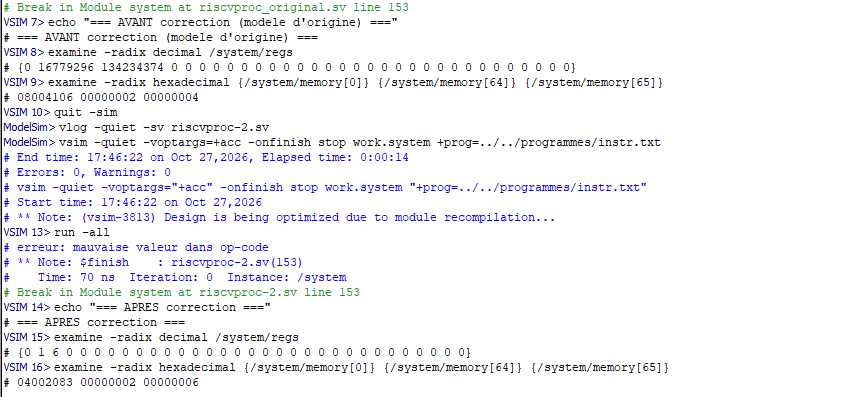
\includegraphics[width=0.98\linewidth]{figures/p4-instr.png}
\caption{Transcript ModelSim : \texttt{instr.txt} avec le modèle d'origine, puis avec le modèle
corrigé}
\label{fig:instr}
\end{figure}

% ---------------------------------------------------------------------------
\subsection{Manipuler les instructions RISC-V (\S\,4.1.1 du sujet)}
\label{sec:codage}

Les instructions RV32I et de l'extension M utilisées ici sont codées sur 32 bits.
Le projet n'utilise pas l'extension C, qui introduit des instructions de 16 bits.
Le modèle utilise trois formats
(tableau~\ref{tab:formats}) : le format R pour les opérations entre registres, le format I pour
les opérations avec un immédiat de 12 bits et pour \texttt{lw}, et le format S pour
\texttt{sw}, dont l'immédiat est découpé en deux champs afin que \texttt{rs1} et \texttt{rs2}
restent à la même place que dans le format R.

\begin{table}[H]
\centering
\begin{tabular}{l|c|c|c|c|c|c|}
\multicolumn{1}{c}{} & \multicolumn{1}{c}{31 -- 25} & \multicolumn{1}{c}{24 -- 20}
 & \multicolumn{1}{c}{19 -- 15} & \multicolumn{1}{c}{14 -- 12} & \multicolumn{1}{c}{11 -- 7}
 & \multicolumn{1}{c}{6 -- 0} \\
\cline{2-7}
R & funct7 & rs2 & rs1 & funct3 & rd & opcode \\
\cline{2-7}
I & \multicolumn{2}{c|}{\texttt{imm[11:0]}} & rs1 & funct3 & rd & opcode \\
\cline{2-7}
S & \texttt{imm[11:5]} & rs2 & rs1 & funct3 & \texttt{imm[4:0]} & opcode \\
\cline{2-7}
\end{tabular}
\caption{Formats d'instructions utilisés (spécification RISC-V, chapitre 2.2)}
\label{tab:formats}
\end{table}

L'instruction \texttt{add x9, x20, x21} est de format R. Ses champs sont donnés dans le
tableau~\ref{tab:add} : le code obtenu est
\texttt{0000 0001 0101 1010 0000 0100 1011 0011}, soit \texttt{0x015A04B3}. L'opcode
\texttt{0110011} désigne les opérations entre registres ; \texttt{funct3} et \texttt{funct7}
choisissent l'opération (\texttt{funct7} vaut \texttt{0100000} pour \texttt{sub}).

\begin{table}[H]
\centering
\begin{tabular}{|c|c|c|c|c|c|}
\hline
funct7 & rs2 = x21 & rs1 = x20 & funct3 & rd = x9 & opcode \\
\hline
\texttt{0000000} & \texttt{10101} & \texttt{10100} & \texttt{000} & \texttt{01001} & \texttt{0110011} \\
\hline
\end{tabular}
\caption{Codage de \texttt{add x9, x20, x21}}
\label{tab:add}
\end{table}

% ---------------------------------------------------------------------------
\subsection{Adapter et implémenter les instructions RISC-V (\S\,4.1.2 du sujet)}
\label{sec:adapter}

\subsubsection{Modes d'adressage}

Le mode d'adressage indique où se trouve l'opérande d'une instruction
(tableau~\ref{tab:adressage}).

\begin{table}[H]
\centering
\begin{tabularx}{\linewidth}{lXl}
\toprule
Mode & Principe & Exemples \\
\midrule
Immédiat & L'opérande est une constante codée dans l'instruction elle-même. & \texttt{addi x1, x0, -7} \\
\addlinespace
Direct & L'adresse mémoire de l'opérande est fixée dans l'instruction ; ici, la base
\texttt{x0} vaut 0. & \texttt{lw x1, 64(x0)} \\
\addlinespace
Indirect & Un registre contient l'adresse de l'opérande en mémoire (pointeur). &
\makecell[tl]{\texttt{lw x1, 0(x2)}\\ \texttt{sw x3, 4(x2)}} \\
\bottomrule
\end{tabularx}
\caption{Modes d'adressage}
\label{tab:adressage}
\end{table}

En RISC-V, \texttt{lw} et \texttt{sw} n'ont qu'un seul mode : l'adresse est la somme d'un
registre de base \texttt{rs1} et d'un déplacement signé de 12 bits, ce qui s'écrit
\texttt{offset(rs1)}. L'adressage direct en est le cas particulier \texttt{rs1} = \texttt{x0} :
\texttt{x0} vaut toujours 0, donc l'adresse 64 de \texttt{lw x1, 64(x0)} est entièrement codée
dans l'instruction. L'adressage indirect en est le cas \texttt{offset} = 0. Dans ce modèle, la
mémoire est adressée par mots de 32 bits (\texttt{memory[addr]}) et non par octets comme dans
la spécification : \texttt{4(x2)} désigne le mot situé 4 mots après l'adresse contenue dans
\texttt{x2}.

\subsubsection{Corrections du modèle fourni}
\label{sec:corrections}

Pour tester les immédiats négatifs, les accès mémoire avec un déplacement positif et négatif,
et le registre \texttt{x0}, nous avons écrit le programme \texttt{test\_base}
(code~\ref{lst:testbase}). Ses résultats sont donnés dans le tableau~\ref{tab:testbase}, relevés
dans ModelSim avec la commande \texttt{examine} (figure~\ref{fig:testbase}) : le modèle d'origine
présente trois erreurs.

\noindent\begin{minipage}{\linewidth}
\begin{lstlisting}[style=code, caption={Programme de test \texttt{test\_base.s}}, label={lst:testbase}]
addi x1, x0, -7      # x1 = -7
addi x2, x0, 100     # x2 = 100
sub  x3, x2, x1      # x3 = 107
andi x4, x1, -16     # x4 = -16
ori  x5, x0, -1      # x5 = -1
addi x6, x0, 3       # x6 = 3
sll  x7, x2, x6      # x7 = 800
srl  x8, x5, x6      # x8 = 0x1FFFFFFF = 536870911
sw   x3, 4(x2)       # mot 104 = 107
sw   x1, -4(x2)      # mot 96 = -7
lw   x9, 4(x2)       # x9 = 107
lw   x10, -4(x2)     # x10 = -7
addi x0, x0, 5       # x0 doit rester a 0
add  x11, x0, x0     # x11 = 0
ebreak
\end{lstlisting}
\end{minipage}\par

\begin{table}[H]
\centering
\begin{tabular}{llrrr}
\toprule
 & Instruction & Attendu & Modèle d'origine & Après correction \\
\midrule
x0  & \texttt{addi x0, x0, 5}   & 0         & 5         & 0 \\
x1  & \texttt{addi x1, x0, -7}  & $-7$      & 4089      & $-7$ \\
x3  & \texttt{sub x3, x2, x1}   & 107       & $-3989$   & 107 \\
x4  & \texttt{andi x4, x1, -16} & $-16$     & 4080      & $-16$ \\
x5  & \texttt{ori x5, x0, -1}   & $-1$      & 4095      & $-1$ \\
x8  & \texttt{srl x8, x5, x6}   & 536870911 & 511       & 536870911 \\
x9  & \texttt{lw x9, 4(x2)}     & 107       & 4089      & 107 \\
x10 & \texttt{lw x10, -4(x2)}   & $-7$      & 4089      & $-7$ \\
x11 & \texttt{add x11, x0, x0}  & 0         & 10        & 0 \\
\midrule
mot 104 & \texttt{sw x3, 4(x2)}  & 107  & \texttt{X} & 107 \\
mot 96  & \texttt{sw x1, -4(x2)} & $-7$ & \texttt{X} & $-7$ \\
mot 0   & première instruction & \texttt{ff900093} & 4089 & \texttt{ff900093} \\
\bottomrule
\end{tabular}
\caption{Résultats de \texttt{test\_base} (x2 = 100, x6 = 3 et x7 = 800 sont corrects dans les deux cas)}
\label{tab:testbase}
\end{table}

\capture[0.8\linewidth]{p4-test-base.png}{Transcript ModelSim, dossier \texttt{exo/p4\_q1} :
\texttt{test\_base} avec le modèle d'origine, puis avec le modèle corrigé}
{Transcript ModelSim : \texttt{test\_base} avec le modèle d'origine, puis avec le modèle
corrigé}{fig:testbase}

Le message \og erreur : mauvaise valeur dans op-code\fg{} affiché au lancement ne vient pas du
programme : ce modèle lit l'instruction par une affectation non bloquante, et l'instruction n'est
pas encore définie à la première période (section~\ref{sec:microarchi}).

\paragraph{Immédiats non étendus en signe.}
Le modèle définissait \lstinline[style=vlinline]|`define I_IMM $signed(instr[31:20])|. Or, en
Verilog, dès qu'un opérande d'une expression est non signé (ici le registre
\texttt{regs[rs1]}), toute l'expression est évaluée en non signé et l'immédiat de 12 bits est
complété par des zéros : $-7$ (\texttt{0xFF9}) devient 4089. C'est l'erreur sur x1, x3, x4 et x5.
Nous faisons l'extension de signe explicitement, en recopiant le bit 31 par concaténation, pour
le format I comme pour le format S (code~\ref{lst:corrections}).

\paragraph{Adresse des accès mémoire.}
L'adresse était calculée par \lstinline[style=vlinline]|addr = `LOAD_OFFSET + regs[`RS1];| avec
\lstinline[style=vlinline]|`define LOAD_OFFSET instr[31:20] << 12|. Une macro est une simple
substitution de texte : la ligne devient
\lstinline[style=vlinline]|addr = instr[31:20] << 12 + regs[`RS1];|, et comme \texttt{+} est
prioritaire sur \lstinline[style=vlinline]|<<|, le déplacement est décalé de 12 + \texttt{rs1} bits. Dans nos
programmes, l'adresse de 12 bits valait donc toujours 0 : les \texttt{lw} lisaient le mot 0 et
les \texttt{sw} écrasaient la première instruction du programme (d'où x9 = x10 = 4089 et le
mot 0 égal à 4089). Le décalage de 12 bits est de toute façon faux : il correspond au format de
\texttt{lui}, pas aux accès mémoire. L'adresse vaut maintenant \texttt{rs1} + immédiat I pour
\texttt{lw}, et \texttt{rs1} + immédiat S pour \texttt{sw}.

\paragraph{Registre x0.}
\texttt{addi x0, x0, 5} modifiait \texttt{x0}, qui doit toujours valoir 0 (spécification,
chapitre 2.1). Nous remettons \texttt{regs[0]} à 0 à la fin de chaque instruction.

\noindent\begin{minipage}{\linewidth}
\begin{lstlisting}[style=verilog, caption={Corrections du modèle (immédiats, adresses, x0)}, label={lst:corrections}]
`define I_IMM   {{20{instr[31]}}, instr[31:20]}               // I-type immediate
`define S_IMM   {{20{instr[31]}}, instr[31:25], instr[11:7]}  // S-type immediate
...
`LW: begin
  addr      = regs[`RS1] + `I_IMM;
  regs[`RD] = memory[addr];
end
...
`SW: begin
  addr         = regs[`RS1] + `S_IMM;
  memory[addr] = regs[`RS2];
end
...
regs[0] = 0;   // x0 is hardwired to 0
\end{lstlisting}
\end{minipage}\par

\subsubsection{Ajout des instructions de l'extension M}
\label{sec:rv32im}

L'extension M ajoute huit instructions de multiplication et de division entières
(tableau~\ref{tab:rv32m}). Ce sont toutes des instructions de format R, avec le même opcode
\texttt{0110011} que \texttt{add} ; elles se distinguent des opérations de RV32I par
\texttt{funct7} = \texttt{0000001} (au lieu de \texttt{0000000} ou \texttt{0100000}), et
\texttt{funct3} choisit l'opération.

\begin{table}[H]
\centering
\begin{tabular}{lcl}
\toprule
Instruction & funct3 & Résultat \\
\midrule
\texttt{MUL}    & \texttt{000} & 32 bits de poids faible de \texttt{rs1} $\times$ \texttt{rs2} \\
\texttt{MULH}   & \texttt{001} & 32 bits de poids fort, signé $\times$ signé \\
\texttt{MULHSU} & \texttt{010} & 32 bits de poids fort, \texttt{rs1} signé $\times$ \texttt{rs2} non signé \\
\texttt{MULHU}  & \texttt{011} & 32 bits de poids fort, non signé $\times$ non signé \\
\texttt{DIV}    & \texttt{100} & quotient signé, arrondi vers 0 \\
\texttt{DIVU}   & \texttt{101} & quotient non signé \\
\texttt{REM}    & \texttt{110} & reste signé, du signe du dividende \\
\texttt{REMU}   & \texttt{111} & reste non signé \\
\bottomrule
\end{tabular}
\caption{Instructions de l'extension M (opcode \texttt{0110011}, funct7 = \texttt{0000001})}
\label{tab:rv32m}
\end{table}

Les modifications à apporter au processeur sont donc les suivantes :
\begin{itemize}
\item \textbf{Décodage} : aucun nouvel opcode n'est nécessaire. Le processeur décode déjà les
opérations entre registres sur le couple \{\texttt{funct3}, \texttt{funct7}\} ; il suffit d'y
ajouter les huit combinaisons.
\item \textbf{Chemin de données} : un multiplieur $32 \times 32$ bits produisant 64 bits, et un
diviseur donnant le quotient et le reste, en versions signée et non signée. Les 32 bits de poids
faible du produit ne dépendent pas du signe des opérandes, d'où une seule instruction
\texttt{MUL} ; les 32 bits de poids fort en dépendent, d'où les trois variantes \texttt{MULH}.
\item \textbf{Cas particuliers} : RISC-V ne déclenche pas d'exception lors d'une division ; la
spécification fixe le résultat de la division par zéro et du dépassement
(tableau~\ref{tab:div0}).
\end{itemize}

\begin{table}[H]
\centering
\begin{tabular}{lcccc}
\toprule
Cas & \texttt{DIV} & \texttt{DIVU} & \texttt{REM} & \texttt{REMU} \\
\midrule
Division par 0 & $-1$ & $2^{32}-1$ & dividende & dividende \\
Dépassement $-2^{31} / (-1)$ & $-2^{31}$ & -- & 0 & -- \\
\bottomrule
\end{tabular}
\caption{Résultats imposés par la spécification pour la division}
\label{tab:div0}
\end{table}

\subsubsection{Implémentation et validation de l'extension M}
\label{sec:rv32im-impl}

Nous avons ajouté les huit codes sous la même forme que les instructions existantes, par exemple
\lstinline[style=vlinline]|`define MUL {3'b000, 7'b0000001}|, et huit cas dans le décodage des
opérations entre registres (code~\ref{lst:rv32m}). Trois points de Verilog demandent de
l'attention :
\begin{itemize}
\item \textbf{Largeur et extension des opérandes.} Dans une affectation directe telle que
\texttt{prod = a * b}, une destination de 64 bits participe au calcul de la largeur de
l'expression : deux opérandes de 32 bits ne provoquent donc pas à eux seuls une troncature
à 32 bits~\cite{systemverilog}. Nos concaténations rendent surtout explicite l'extension
voulue pour chaque opérande : copie du signe avec
\lstinline[style=vlinline]|{{32{x[31]}}, x}| ou ajout de zéros avec
\lstinline[style=vlinline]|{32'b0, x}|. Le produit est conservé sur 64 bits dans
\texttt{prod}, puis les bits 63 à 32 sont copiés pour les variantes \texttt{MULH}.
\item \textbf{Division signée.} Les deux opérandes passent par \texttt{\$signed}. La division
signée de Verilog arrondit vers zéro et le reste prend le signe du dividende, comme en RISC-V.
\item \textbf{Cas particuliers.} En Verilog, une division par zéro donne \texttt{X} ; ces cas sont
donc traités avant la division, avec \texttt{if}/\texttt{else}. Nous avons évité l'opérateur
conditionnel \texttt{? :} : si l'une de ses branches est non signée (par exemple
\texttt{32'hFFFFFFFF}), toute l'expression devient non signée, et la division de l'autre branche
est alors calculée en non signé ($-7 / 2$ donne 2147483644 au lieu de $-3$).
\end{itemize}

\noindent\begin{minipage}{\linewidth}
\begin{lstlisting}[style=verilog, caption={Extrait de l'implémentation de l'extension M}, label={lst:rv32m}]
reg[63:0] prod;   // 64-bit product for MULH, MULHSU, MULHU
...
`MUL:    regs[`RD] = regs[`RS1] * regs[`RS2];  // 32-bit target: low half
`MULH:   begin
           prod = {{32{regs[`RS1][31]}}, regs[`RS1]} * {{32{regs[`RS2][31]}}, regs[`RS2]};
           regs[`RD] = prod[63:32];
         end
...
`DIV:    if (regs[`RS2] == 0)
           regs[`RD] = 32'hFFFFFFFF;                     // division by 0: -1
         else if (regs[`RS1] == 32'h80000000 && regs[`RS2] == 32'hFFFFFFFF)
           regs[`RD] = 32'h80000000;                     // overflow: -2^31
         else
           regs[`RD] = $signed(regs[`RS1]) / $signed(regs[`RS2]);
\end{lstlisting}
\end{minipage}\par

Le programme \texttt{test\_rv32im} teste les huit instructions et les trois cas particuliers.
Avant la modification, le processeur affichait onze fois \og erreur : mauvaise instruction
arithmétique\fg{}, une fois par instruction de l'extension M, et les registres correspondants
restaient à 0 (figure~\ref{fig:rv32im-avant}). Après la modification, toutes les valeurs sont
celles attendues (tableau~\ref{tab:rv32imres} et figure~\ref{fig:rv32im}).

\capture[0.82\linewidth]{p4-rv32im-avant.png}{Transcript ModelSim, dossier \texttt{exo/p4\_q1} :
\texttt{test\_rv32im} avant l'ajout de l'extension M}
{Transcript ModelSim : \texttt{test\_rv32im} avant l'ajout de l'extension M (le transcript
affiche mal l'accent de \og arithmétique\fg{})}{fig:rv32im-avant}

\begin{table}[H]
\centering
\begin{tabular}{llrl}
\toprule
Instruction & Registre & Résultat & Remarque \\
\midrule
\texttt{mul x3, x1, x2}     & x3  & $-14$ & \\
\texttt{div x4, x1, x2}     & x4  & $-3$  & arrondi vers 0 \\
\texttt{rem x5, x1, x2}     & x5  & $-1$  & signe du dividende \\
\texttt{divu x6, x1, x2}    & x6  & 2147483644 & \texttt{0xFFFFFFF9} / 2 \\
\texttt{div x7, x1, x0}     & x7  & $-1$  & division par 0 \\
\texttt{mulh x8, x1, x2}    & x8  & $-1$  & partie haute de $-14$ \\
\texttt{mulhu x9, x1, x2}   & x9  & 1     & \texttt{0xFFFFFFF9} $\times$ 2 = \texttt{0x1FFFFFFF2} \\
\texttt{remu x10, x1, x2}   & x10 & 1     & \\
\texttt{mulhsu x16, x1, x2} & x16 & $-1$  & \\
\texttt{div x14, x11, x12}  & x14 & $-2^{31}$ & dépassement \\
\texttt{rem x15, x11, x12}  & x15 & 0     & dépassement \\
\bottomrule
\end{tabular}
\caption{Résultats de \texttt{test\_rv32im}, avec x1 = $-7$, x2 = 2, x11 = $-2^{31}$ et x12 = $-1$}
\label{tab:rv32imres}
\end{table}

\capture{p4-rv32im.png}{Transcript ModelSim, dossier \texttt{exo/p4\_q2} : registres après
\texttt{test\_rv32im}}
{Transcript ModelSim : registres après \texttt{test\_rv32im}}{fig:rv32im}

% ---------------------------------------------------------------------------
\subsection{Adapter la micro-architecture du processeur RISC-V (\S\,4.2 du sujet)}
\label{sec:microarchi}

Pour pouvoir relier le processeur au bloc \texttt{quadram}, le module \texttt{system}, qui
n'avait pas de port, devient le module \texttt{riscvproc} avec une horloge, un reset et un bus de
données (tableau~\ref{tab:ports}). L'adresse fait 12 bits, comme le bus d'adresse interne du
processeur : elle désigne 4096 mots, soit les 4 RAM de 1024 mots de la
partie~\ref{sec:systeme}.

\begin{table}[H]
\centering
\begin{tabular}{llcl}
\toprule
Port & Direction & Largeur & Rôle \\
\midrule
\texttt{clock}       & entrée & 1  & horloge \\
\texttt{reset}       & entrée & 1  & remise à zéro synchrone, active à 1 \\
\texttt{address}     & sortie & 12 & adresse du mot de données \\
\texttt{dataToWrite} & sortie & 32 & donnée à écrire \\
\texttt{dataToRead}  & entrée & 32 & donnée lue \\
\texttt{we}          & sortie & 1  & autorisation d'écriture \\
\bottomrule
\end{tabular}
\caption{Ports ajoutés au processeur}
\label{tab:ports}
\end{table}

Les autres modifications sont les suivantes (code~\ref{lst:horloge}) :
\begin{itemize}
\item \textbf{Horloge.} Le paramètre \texttt{Step} et l'attente \texttt{\#Step} sont remplacés
par \lstinline[style=vlinline]|@(negedge clock)| : le processeur exécute une instruction par
période d'horloge, sur le front descendant. Le bloc \texttt{quadram} échantillonne ses entrées
sur le front montant, une demi-période plus tard : les signaux du bus sont alors stables.
\item \textbf{Reset synchrone}, actif à 1 : sur un front descendant avec \texttt{reset} = 1,
\texttt{pc} et les registres reprennent leur valeur initiale, 0. La mémoire programme n'est pas
modifiée.
\item \textbf{Lecture de l'instruction par affectation bloquante.} Le modèle d'origine utilisait
\lstinline[style=vlinline]|instr <= memory[pc];|. Avec une affectation non bloquante,
\texttt{instr} n'est mise à jour qu'après le décodage, si bien que chaque période décodait
l'instruction lue à la période précédente ; à la première période, l'instruction était encore
indéfinie, d'où un message \og mauvaise valeur dans op-code\fg{} au démarrage. Avec
\lstinline[style=vlinline]|instr = memory[pc];|, l'instruction est lue et exécutée dans la même
période. C'est aussi nécessaire pour la partie~\ref{sec:systeme}, où \texttt{lw} et \texttt{sw}
attendent la mémoire alors que \texttt{instr} doit rester stable.
\item \textbf{Sorties du bus} initialisées à 0 : à cette étape, les données sont encore dans la
mémoire interne.
\end{itemize}

\noindent\begin{minipage}{\linewidth}
\begin{lstlisting}[style=verilog, caption={Boucle principale du processeur avec horloge et reset}, label={lst:horloge}]
always begin // one instruction per clock period
  @(negedge clock);
  if (reset) begin
    // synchronous reset: same values as at the start of the simulation
    pc = 0;
    for (index = 0; index < NRegs; index = index + 1) begin
      regs[index] = 0;
    end
  end else begin
    instr = memory[pc];   // instruction fetch (blocking: executed in this same period)
    pc    = pc + 1;       // increment program counter
    addr  = 0;            // address initial value
    case(`OPCODE)         // decode instruction
      ...
    endcase
    regs[0] = 0;
  end // if (reset) ... else
end
\end{lstlisting}
\end{minipage}\par

Le testbench \texttt{tb\_riscvproc.sv} instancie le processeur, génère une horloge de période
10~ns et maintient le reset à 1 jusqu'à 12~ns, ce qui laisse un front descendant de reset à
10~ns. La première instruction est exécutée à 20~ns, puis une instruction toutes les 10~ns.
Sur la figure~\ref{fig:horloge}, les curseurs marquent la fin du reset (12~ns), la première
instruction (20~ns) et la fin de la simulation (190~ns). Les 170~ns qui séparent la première
et la dernière des 18 instructions de \texttt{test\_rv32im} représentent 17 périodes : une
instruction par période. Les résultats sont identiques à ceux de la section précédente :
\texttt{test\_rv32im} se termine à 190~ns, \texttt{test\_base} à 160~ns, \texttt{instr.txt} et
\texttt{instr2.txt} à 70~ns (figure~\ref{fig:horloge-prog}).

\capture{p4-horloge.png}{ModelSim, dossier \texttt{exo/p4\_q3}, programme \texttt{test\_rv32im} :
signaux \texttt{clock}, \texttt{reset}, \texttt{pc} et \texttt{instr} de 0 à 190~ns}
{Processeur avec horloge et reset, programme \texttt{test\_rv32im} : une instruction par
période}{fig:horloge}

\capture[0.85\linewidth]{p4-horloge-programmes.png}{Transcript ModelSim, dossier
\texttt{exo/p4\_q3} : \texttt{test\_base}, \texttt{instr.txt} puis \texttt{instr2.txt}}
{Transcript ModelSim : processeur avec horloge, programmes \texttt{test\_base},
\texttt{instr.txt} puis \texttt{instr2.txt}}{fig:horloge-prog}
